
\chapter{Σχεδιασμός} % Main chapter title

\label{Σχεδιασμός} % Change X to a consecutive number; for referencing this chapter elsewhere, use \ref{ChapterX}

\lhead{Κεφάλαιο 3. \emph{Σχεδιασμός}} % Change X to a consecutive number; this is for the header on each page - perhaps a shortened title


%----------------------------------------------------------------------------------------
%	SECTION 1
%----------------------------------------------------------------------------------------


\section{socialPServer}
\noindent
Όπως προαναφέρθηκε, η προσέγγιση που ακολουθάτε στην παρούσα εργασίας αφορά την επέκταση ενός συστήματος συστάσεων ώστε να μπορεί να εξάγει συμπεράσματα για τους χρήστες του μελετώντας τον κοινωνικό τους γράφο.
Με αυτό τον τρόπο θα βελτιωθεί η ακρίβεια των συστάσεων με παραδοχή πως οι χρήστες τείνουν να έχουν κοινά ενδιαφέροντα και προτιμήσεις
με τους ανθρώπους τους οποίους έχουν επιλέξει να είναι κοινωνικά συνδεδεμένοι.
Αυτό πρακτικά σημαίνει πως έχοντας κάποιας μορφής κοινωνικό γράφο μπορούν να ομαδοποιηθούν τα μέλη του (χρήστες) σύμφωνα
με τις ακμές φιλίας ή εμπιστοσύνης που τους ενώνουν. Εντοπίζονται δηλαδή ομάδες (communities) \emph{στενά συνδεδεμένων χρηστών}
οι οποίες αποτελούν πηγή εξόρυξης διαφόρων τύπων δεδομένων. Συγκεκριμένα, πρόκειται να αξιοποιηθεί η ύπαρξη κάποιου χρήστη
σε κάποια κοινωνική ομάδα για να σκιαγραφηθούν οι προτιμήσεις του.

Το πρόγραμμα που υλοποιήθηκε για την επίτευξη των παραπάνω \setlanguage{english} \emph{(social PServer)} \setlanguage{greek} έχει τους παρακάτω \textbf{στόχους}:

\begin{description}
\item \textbf{Να αποτελέσει μια πλατφόρμα στην οποία μπορούν να ενσωματωθούν αλγόριθμοι παραγωγής κοινοτήτων χρηστών δοσμένου ενός κοινωνικού γράφου.}  \hfill \\
Επομένως πρέπει να περιλαμβάνονται όλες οι απαραίτητοι μέθοδοι για τον χειρισμό τον δεδομένων και την ολοκλήρωση της διαδικασίας διατηρώντας μια εσωτερική αυτονομία των λειτουργιών.
Αυτό επιτυγχάνεται διατηρώντας σαφή είσοδο και έξοδο της κάθε διαδικασίας και δημιουργώντας τα κατάλληλα \emph{interfaces} που θα λειτουργήσουν σαν πρότυπα-οδηγοί για την προσθήκη
νέων αλγορίθμων.
\item \textbf{Να εγκατασταθεί ένας αριθμός αλγορίθμων στο πρόγραμμα.}  \hfill \\
Ώστε να δοκιμαστεί η διαδικασία αλλά κυρίως για να αποκτήσει λειτουργικότητα. Η ενσωμάτωση αλγορίθμων στο πρόγραμμα το καθιστά πλέον όντος μια μηχανή εντοπισμού
κοινοτήτων η οποία είναι εργαλείο για ανάλυση κοινωνικών δικτύων και μπορεί να εφαρμοστεί σε πληθώρα εφαρμογών από την κοινωνιολογία, ως την στοχευμένη διαφήμιση.
\item \textbf{Να ενσωματωθεί στο υπάρχον Recomendation System PServer}  \hfill \\
Να χρησιμοποιηθεί δηλαδή το πρόγραμμά μας για να επεκτείνει την λειτουργία του PServer επιτρέποντας του να παρέχει προσωποποίηση αναλύοντας τον κοινωνικό γράφο των χρηστών του.
\end{description} 


\begin{figure}[htbp]
  \begin{center}
  %\hspace{-4.0em}    
    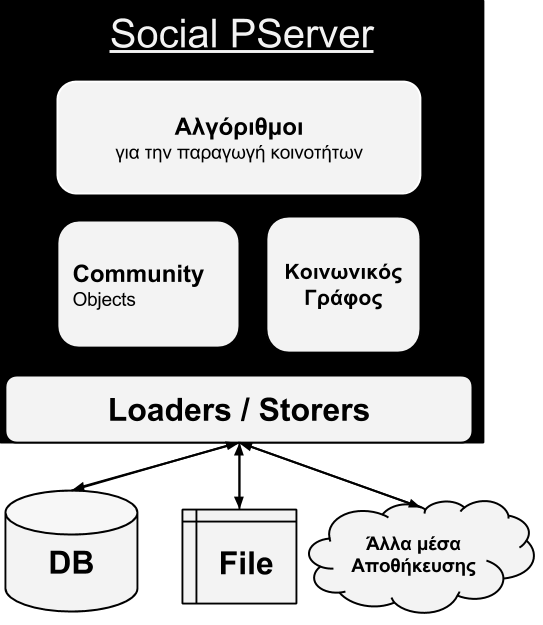
\includegraphics[scale=0.60]{Figures/socialPServerComponents.png}
	\rule{35em}{0.5pt}  % UnderLine figure	
	\caption[PServerArchitecture]{Η εσωτερική οργάνωση του socialPServer}
  \end{center}	
  \label{fig:socialPServerComponents}  
\end{figure}

\vfill

\section{Κοινωνική Πληροφορία}
\noindent
Αρχικό βήμα για την επίλυση του προβλήματος είναι να μπορούν να διαβαστούν και να επεξεργαστούν οι κοινωνικές πληροφορίες.
Το ποιες πληροφορίες πρέπει να συλλεχθούν στην την κάθε περίπτωση εξαρτάται από τη φύση αλλά και τους στόχος της υπηρεσίας.
Η συλλογή αυτών δεν αφορά τον socialPServer αλλά πραγματοποιείται από την εκάστοτε υπηρεσία. 
Κοινωνική συσχέτιση μπορεί να σημαίνει ξεκάθαρη δήλωση φιλίας από τον χρήστη άλλα μπορεί και να εντοπίζεται μέσα από την
αλληλεπίδραση του χρήστη με το σύστημα. Δηλαδή η κοινωνική πληροφορία μπορεί να εκφράζει διαφορετικά πράγματα,
αλλά αυτό που σε κάθε περίπτωση έχει ενδιαφέρον είναι η αξιοποίηση της κοινωνικής διασύνδεσης.

Η σχέση μεταξύ δυο χρηστών μπορεί να έχει διάφορες μορφές και χαρακτηριστικά. Μπορεί να είναι να έχει κατεύθυνση (directed) που σημαίνει πως κάποιος χρήστης
εμπιστεύεται κάποιον άλλον όμως μπορεί να μην συμβαίνει το αντίθετο, μπορεί να έχει κάποιο βάρος (weighted) το οποίο υποδηλώνει τον βαθμό
φιλίας των δύο ή μπορεί και να είναι undirected και unweighted να δηλώνει δηλαδή απλά την συσχέτιση δύο χρηστών. Στην τελευταία αυτή κατηγορία
έγκειται και το πρόγραμμά που υλοποιήσαμε (socialPServer) ο οποίος αποθηκεύει την εκάστοτε φιλία στην Βάση Δεδομένων καταχωρώντας μία εγγραφή τα userIDs των δύο εμπλεκόμενων χρηστών.


\subsection*{Κοινωνικός Γράφος}
\noindent
Σε αυτό το σημείο, έχοντας λοιπόν την κοινωνική πληροφορία, αρχίζει η λειτουργία του socialPServer. Το πρώτο πράγμα που πρέπει να γίνει
είναι η ανάκτηση των δεδομένων φιλίας και η δημιουργία μιας δομής δεδομένων η οποία να αντιπροσωπεύει έναν εικονικό κοινωνικό γράφο.
Για λόγους τόσο ευχρηστίας αλλά και αποδοτικότητας, για τον χειρισμό των γράφων, χρησιμοποιούνται open-source java βιβλιοθήκες στοχευμένες σε αυτό. Στη συνέχεια λοιπόν
ανάλογα με τον αλγόριθμο που θα χρησιμοποιηθεί για την παραγωγή κοινοτήτων, χρησιμοποιείται και η κατάλληλη κοινωνική δομή - γράφος.



\section{Κοινότητες χρηστών}
\noindent
Με την εφαρμογή των αλγορίθμων πρόκειται να εντοπιστούν σύνολα χρηστών τα οποία μπορούν να χαρακτηριστούν κοινότητες. Για να είναι αυτή η γνώση αξιοποιήσιμη,
σε κάθε μία από αυτές δίνεται ένα ID και στην συνέχεια για κάθε μέλος ομάδας, αποθηκεύεται στην Βάση μια εγγραφή που φέρει το UserID και το ComminityID. Με αυτόν το τρόπο μπορεί ο διαχειριστής της εκάστοτε υπηρεσίας
με μία ερώτηση στη βάση (query) να γνωρίζει ποιοι χρήστες αποτελούν ομάδα, ποιος είναι ο κοινωνικός κύκλος του κάθε χρήστη και λοιπές πληροφορίες.

\section{Προφίλ Χρήστη (userProfile)}
\noindent
Για να μπορούμε τελικός να παραχθούν συστάσεις, πρέπει εκτός από την κοινωνική πληροφορία να είναι γνωστές και οι προτιμήσεις των χρηστών, που είναι οι υπάρχουσες αξιολογήσεις αντικειμένων. 
Επομένως πρέπει να υπάρχει ένα \emph{προφίλ χρήστη} το οποίο θα περιέχει τις κάθε φορά απαραίτητες πληροφορίες 
που μας επιτρέπουν να σκιαγραφήσουμε τα ενδιαφέροντα και την συμπεριφορά του. Στην περίπτωσή μας αυτή η διαδικασία πραγματοποιείται είδη στον PServer, 
αφού πρόκειται για μια υπάρχουσα, λειτουργική και εφαρμοσμένη μηχανή προσωποποίησης. Συγκεκριμένα το \emph{user profile} περιλαμβάνει πληροφορίες για τις προτιμήσεις των χρηστών αλλά και
για τα δημογραφικά τους χαρακτηριστικά. Στα πλαίσια αυτής της εργασίας χρησιμοποιούμε τις πληροφορίες των προφίλ για να αξιολογούμε την διαδικασία παραγωγής κοινοτήτων χρησιμοποιώντας 
υπάρχοντα δεδομένα (εσωτερική αξιολόγηση). Οι προτιμήσεις των χρηστών θα ξαναχρησιμοποιηθούν όταν θα γίνουν τελικά οι συστάσεις αλλά αυτό όπως φαίνεται και από την παραπάνω περιγραφή του συστήματος, είναι 
λειτουργία του εκάστοτε recommendation engine που ανάλογα με την περίπτωση θα υπολογίσει τις πιθανές αξιολογήσεις.

\section{PServer}
\label{PServer}
\noindent
Σε αυτό το σημείο θα δοθεί περαιτέρω εξήγηση για την υπάρχουσα πλατφόρμα την οποία καλείτε να επεκτείνει το δικό μας πρόγραμμα. 
Ο PServer\cite{pServer} είναι ένας γενικής χρήσης \emph{personalization Server} οποίος είχε αναπτυχθεί από το ερευνητικό κέντρο \textbf{Δημόκριτος} και στην συνέχεια από τον οργανισμό \textbf{SciFY}.
Επόμενος πρόκειται για να λειτουργικό πρόγραμμα που μπορεί να εγκατασταθεί σε διαφορετικών ειδών εφαρμογές
για να προσφέρει προσωποποιημένη υπηρεσία. Με τον όρο προσωποποίηση εννοούμε διαφοροποίηση του περιεχομένου μιας υπηρεσίας ανάλογα με τις προτιμήσεις και την αισθητική του κάθε χρήστη.
\cite{pServerUserGuide}\\
Προσωποποίηση επιτυγχάνεται με διαφορετικούς τρόπους όπως εμφάνιση διαφορετικού GraphicalUserInterface σε κάθε χρήστη ώστε να είναι 
προσιτό σε αυτόν, προβολή διαφημίσεων που αφορούν μόνο αντικείμενα για τα οποία χρήστης έχει δείξει ενδιαφέρον στο παρελθόν και άλλους. 
Ο PServer περιλαμβάνει τις λειτουργίες που χρειάζονται για να υπάρξει ένα σύστημα συστάσεων. Αποτελεί δηλαδή την μηχανή η οποία θα αναλάβει να 
να οργανώσει τα προφίλ των χρηστών και να τους κατηγοριοποιήσει ώστε να μπορέσουν να εξαχθούν συμπεράσματα για τις προτιμήσεις τους.\\



Η λειτουργία του περιλαμβάνει τα εξής λογικά επίπεδα. 
\begin{description}
\item \textbf{Personal user models}  \hfill \\
Είναι ουσιαστικά οι πληροφορίες που αποθηκεύονται για κάθε χρήστη ώστε να μπορεί να δημιουργηθεί 
ένα user profile. Μπορεί να είναι δημογραφικά χαρακτηριστικά (\emph{Attributes} - πχ. ηλικία, φύλο) ή πληροφορίες περιεχομένου
(\emph{Features}) που αναφέρονται στην οντολογία της κάθε εφαρμογής (πχ αξιολογήσεις αντικειμένων).
\item \textbf{Stereotypes}  \hfill \\
Είναι ομάδες χρηστών με κοινά δημογραφικά χαρακτηριστικά (Attributes), οι οποίες παράγονται από τον PServer. 
\item \textbf{User Communities}  \hfill \\
Ομάδες χρηστών που προκύπτουν από την αλληλεπίδρασή τους με το σύστημα. Προς το παρόν οι χρήστες ομαδοποιούνται από 
τον PServer με βάσει τα Feature τους.
Σε αυτό το λογικό επίπεδο ανήκει και το πρόγραμμά μας, το οποίο πρόκειται να εντοπίζει τέτοιου είδους
ομάδες μελετώντας την κοινωνική συσχέτιση των χρηστών.
\end{description} 
\cite{pServerUserGuide}

\section{Αρχιτεκτονική του PServer}
\noindent
Ο PServer έχει σχεδιαστεί ώστε να είναι ανεξάρτητος από την υπηρεσία και την πλατφόρμα, με την έννοια ότι
μπορεί να λειτουργήσει σε διαφορετικά Λειτουργικά Συστήματα και μπορεί να προσφέρει υπηρεσίες προσωποποίησης 
σε κάθε εφαρμογή ανεξαρτήτως περιεχομένου. Για την επίτευξη των παραπάνω, η υλοποίησή του έχει γίνει σε java
χωρίς καθόλου χρήση API του λειτουργικού συστήματος. Το μόνο που απαιτείται είναι το μηχάνημα να διαθέτει
ένα port με Java virtual machine version 1.5+. Επίσης για να λειτουργήσει χρειάζεται μία 
σχεσιακή βάση δεδομένων, συγκεκριμένα χρησιμοποιεί MySQL 5+, η οποία είναι ανοιχτού κώδικα και 
λειτουργεί σε όλα τα διαδεδομένα Λειτουργικά Συστήματα. Τέλος για να διατηρεί ανεξαρτησία από την 
πλατφόρμα είναι σχεδιασμένος ώστε να επικοινωνεί χρησιμοποιώντας HTTP πρωτόκολλο.
Δέχεται Http requests από τις εφαρμογές που εξυπηρετεί, τα οποία περιλαμβάνουν εντολές και παραμέτρους και δίνει απάντηση σε μορφή XML ή JSON.
\cite{pServerUserGuide}

Ο PServer μπορεί να εξυπηρετεί ταυτόχρονος πολλές WEB υπηρεσίες τις οποίες ξεχωρίζει με ένα \emph{ClientID}.
Κάθε εγγραφή που αποθηκεύεται στην βάση έχει και μια στήλη με αυτό το χαρακτηριστικό ώστε να ξεχωρίζεται το περιεχόμενο των διαφορετικών πελατών του.
Σε κάθε HTTP request, εμπεριέχονται επίσης το ClientID ένας κωδικός για την αυθεντικοποίηση της υπηρεσίας.

Κάθε υπηρεσία κάνει διαφορετικές ενέργειες ώστε να προσωποποιήσει το περιεχόμενό της. 
Αυτό που προσφέρει ο PServer είναι οι απαραίτητες πληροφορίες που απαιτούνται για να υπάρξει ένα σύστημα προσωποποίησης. 
Για να μπορέσει μια υπάρχουσα υπηρεσία να εκμεταλλευτεί την λειτουργία του, 
πρέπει να υλοποιηθεί ένα ενδιάμεσο επίπεδο επικοινωνίας μεταξύ του PServer και της υπηρεσίας που ονομάζεται \textbf{Recommendation Engine},
του οποίου ο σχεδιασμός εξαρτάται κάθε φορά από τους στόχους της εφαρμογής.
Αυτό το επίπεδο αναλαμβάνει να τον τροφοδοτεί με δεδομένα, να δώσει τις σχετικές εντολές που χρειάζονται για την παραγωγή Στερεοτύπων και Κοινοτήτων 
και να ανακτήσει πληροφορίες από αυτόν. Επίσης εδώ θα προεπεξεργαστούν οι πληροφορίες που επιστρέφει ο PServer, ώστε να έχουν νόημα για την εκάστοτε υπηρεσία.


\begin{figure}[htbp]
  %\begin{center}
  \hspace{-3.5em}  
    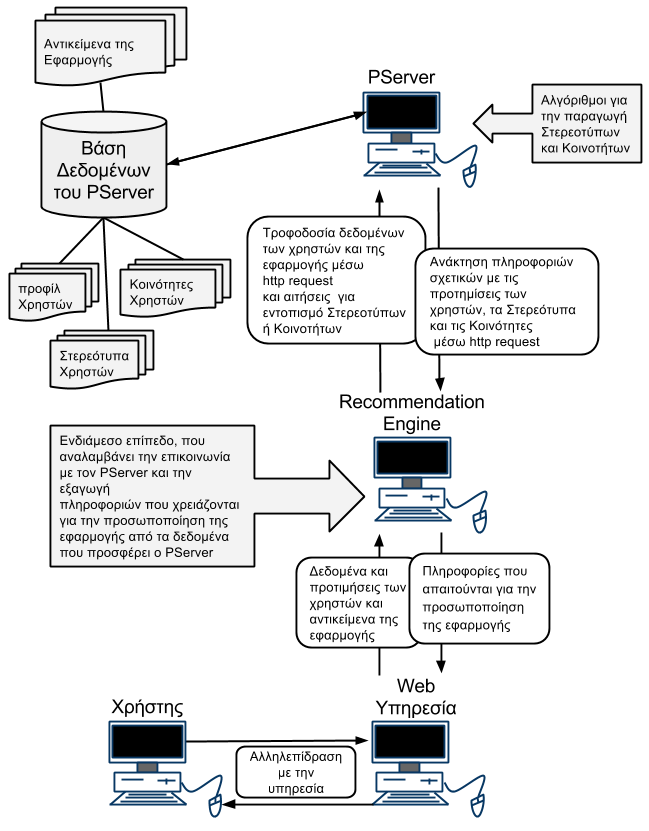
\includegraphics[scale=0.75]{Figures/PServerArchitecture.png}
	\rule{35em}{0.5pt}  % UnderLine figure	
	\caption[PServerArchitecture]{Η αρχιτεκτονική του PServer}
 % \end{center}	
  \label{fig:PServerArchitecture}  
\end{figure}


\vfill

\section{ενσωμάτωση στον PServer}

\noindent
Σημαντικός παράγοντας της αρχιτεκτονικής του προγράμματός μας είναι η αυτονομία και η μεταφερσιμότητα, ώστε να μπορεί να συμπεριληφθεί σε οποιαδήποτε άλλη java εφαρμογή σαν βιβλιοθήκη.
Έτσι και στην περίπτωση του PServer ενσωματώθηκε σαν βιβλιοθήκη και για να γίνει χρήση των λειτουργιών του καλείται με τις ανάλογες παραμέτρους που αφορούν την επιλογή του αλγορίθμου και τις
παραμέτρους αυτού.

Η λειτουργία του socialPServer απαιτεί ένα μέσο αποθήκευσης Δεδομένων στο οποίο να εμπεριέχονται τα στοιχεία των χρηστών και της εφαρμογής,
επομένως κατά την εγκατάστασή του σε κάποιο μηχάνημα ο προγραμματιστής δημιουργεί την σχετική Βάση Δεδομένων ή κάποιου τύπου αρχείο με τις απαραίτητες πληροφορίες.
Εφόσον σκοπός είναι να επεκταθούν οι υπάρχουσες λειτουργίες του PServer καλύτερο θα ήταν να χρησιμοποιεί κοινή Βάση Δεδομένων με αυτόν. 
Για να μπορούν λοιπόν να συνεργάζονται σε επίπεδο δεδομένων, στο πρόγραμμά μας χρησιμοποιούνται οι υπάρχουσες μέθοδοι που είναι υλοποιημένες στον pServer για την αλληλεπίδραση με την Βάση.
Επομένως δημιουργήσαμε ένα ενδιάμεσο επίπεδο που μεταφράζει την επικοινωνία μας με την Βάση στις μεθόδους επικοινωνίας του PServer. 
Πρακτικά λοιπόν όταν ο pServer καλεί το πρόγραμμά μας δίνει ως παράμετρο και 
ένα αντικείμενο της κλάσης του \emph{DBAccess} το οποίο περιλαμβάνει μεθόδους για τον χειρισμό των πινάκων με τους οποίους λειτουργεί.
Αυτό το αντικείμενο δίνουμε κατά την αρχικοποίηση στην δικιά μας ενδιάμεση κλάση η οποία θα αναλάβει να μεταφράζει όλες τις επικοινωνίες 
του προγράμματός μας σε επικοινωνίες του pServer.

Τέλος, στην πλευρά του PServer, προστέθηκαν κάποιες λειτουργίες στο API του χρησμού του,
ώστε να μπορεί η κάθε υπηρεσία που τον χρησιμοποιεί να τον τροφοδοτήσει με την 
απαραίτητη πληροφορία φιλίας αλλά και να χρησιμοποιεί τους Αλγορίθμους του.\\
Συγκεκριμένα ο PServer ενημερώθηκε καταλλήλως για να μπορεί να δεχτεί αιτήσεις που δηλώνουν την φιλία χρηστών και αιτήσεις
για παραγωγή κοινοτήτων χρηστών με βάση την κοινωνική πληροφορία.


\begin{figure}[htbp]
  %\begin{center}
  \hspace{-8.5em}  
    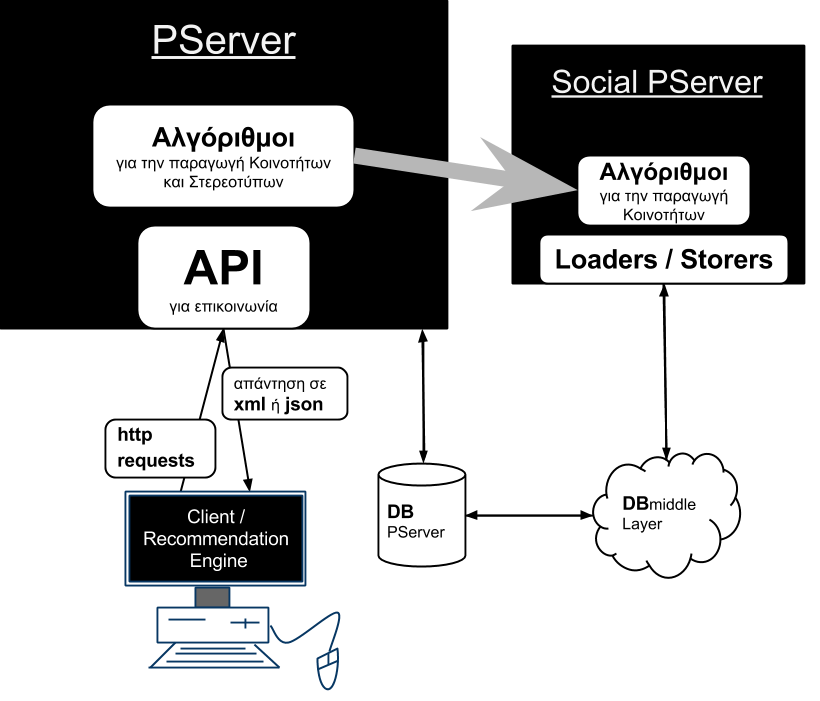
\includegraphics[scale=0.70]{Figures/socialPServer_PServer_combine.png}
	\rule{35em}{0.5pt}  % UnderLine figure	
	\caption[PServerArchitecture]{ενσωμάτωση του socialPServer στον PServer\\
	Το βέλος που ενώνει τους δυο μηχανισμούς Αλγορίθμων συμβολίζει την περίπτωση
	που ο Client, μέσω του API, ζητά τον εντοπισμό κοινοτήτων με βάση τους κοινωνικούς δεσμούς
	και επομένως\\ ο PServer καλεί τον socialPServer}
 %\end{center}	
  \label{fig:socialPServer_PServer_combine}  
\end{figure}


